\section{Übersicht der Systemarchitektur}
\begin{figure}[h]
    \centering
    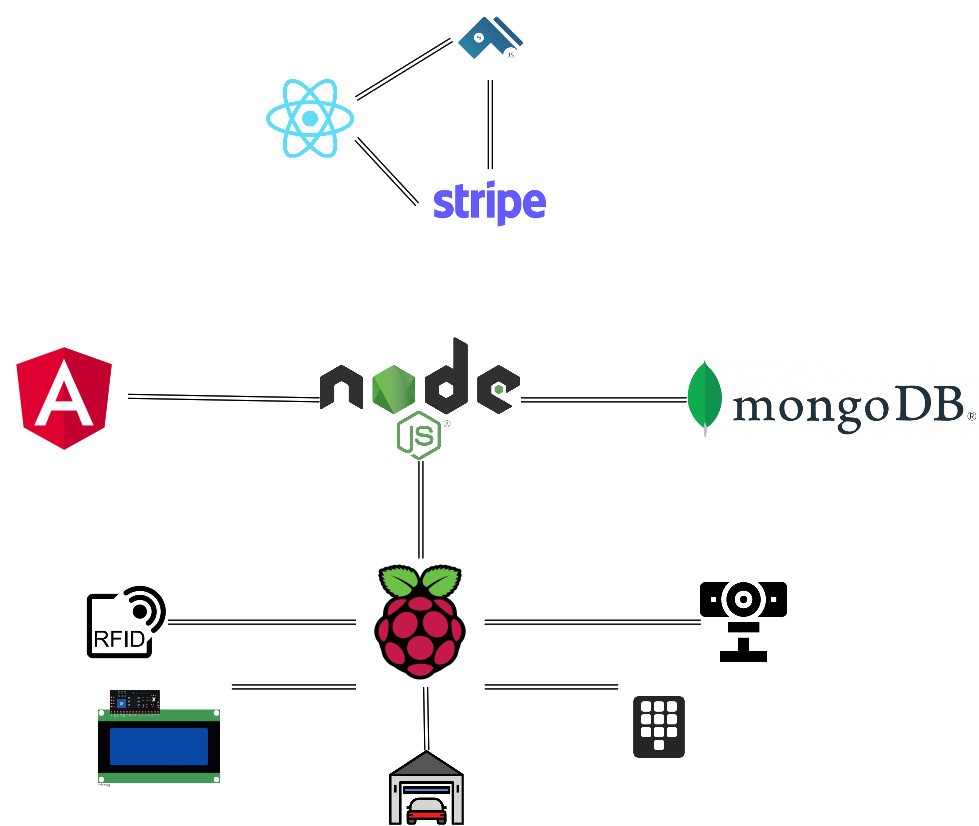
\includegraphics[width=10cm]{pics/APERTASystemarchitektur.jpg}
    \caption{Systemarchitektur}
    \end{figure}
Diese Diplomarbeit setzt sich aus zwei voneinander unabhängigen Systemen zusammen. Das Shopsystem, bestehend aus einem React-Frontend, kommuniziert mit zwei Bibliotheken, CommerceJS und Stripe, welche für die Produktverwaltung, sowie den Bezahlvorgang zuständig sind. Das Angular-Frontend des Dashboard in Verbindung mit dem NodeJS Server, der MongoDB Datenbank sowie dem Raspberry bietet das zweite System.
Der Raspberry ist über GPIOs mit dem RFID-Leser, dem Nummernfeld und dem Display verbunden. Weiters wurde die Kamera an einen der USB 3.0 Ports des Raspberry angeschlossen.
\section{Frontend (Angular-Applikation)}
\setauthor{David Hauser}

\section{Frontend (React-Applikation)}
\setauthor{Benjamin Golic}

\section{Backend (NodeJS-Server)[SK]}
\setauthor{Simon Koll}
Das Backend besteht aus einer JavaScipt Datei, in welcher sämtliche Endpunkte definiert werden. Weiters benötigt das Backend einige Pakete, um beispielsweise mit der Datenbank zu kommunizieren. Diese werden in \verb|package.json| aufgeführt. Bei erstmaliger Installation wird die Datei automatisch durchlaugfen, und installiert alle benötigten Dateien und Pakete. Dazu wird der Terminal-Befehl \verb|npm install| ausgeführt. Der Node Package Manager installiert alle Pakete im Ordner \verb|node_modules|.\\
Der Server selbst wird weiters eingeteilt in:

\begin{itemize}
    \item \textit{Imports: } Zu beginn werden alle benötigten Pakete importiert. Dies geschiet mittels \verb|require()|.
    \item \textit{Setup:  } In weiterer Folge werden benötigte Variablen, wie die Verbindungs-URL der MongoDB Datenbank, definiert. Da die Datenbank und der Server auf der selben Maschine laufen, der Host auf \verb|mongodb://127.0.0.1:27017| gesetzt. Der weitere Aufbau der UTL besteht aus Parametern wie zum Beispiel der \verb|serverSelectionTimeOutMS|.
    \item \textit{Header: } Um den Zugriff des Raspberry auf den Server zu gewährleisten, müssen die Header-Parameter gesetzt werden. Dies geschieht mittels \verb|app.use()| und einer als Parameter übergebenen Funktion, in der mit \verb|res.setHeader()| die Header-Parameter gesetzt werden. Diese bestimmen welche IP-Adressen auf den Server zugreifen können, welche Methoden verwedet werden dürfen, sowie die zugelassenen Header bei Anfragen des Clients.
\end{itemize}
\section{Kennzeichenerkennung [SK]}
\setauthor{Simon Koll}
